%%%% ijcai19-multiauthor.tex

\typeout{IJCAI-19 Multiple authors example}

% These are the instructions for authors for IJCAI-19.

\documentclass{article}
\pdfpagewidth=8.5in
\pdfpageheight=11in
% The file ijcai19.sty is NOT the same than previous years'
\usepackage{../ijcai19}

% Use the postscript times font!
\usepackage{times}
\usepackage{soul}
\usepackage[hyphens]{url}
\usepackage[hidelinks]{hyperref}
\usepackage[utf8]{inputenc}
\usepackage[small]{caption}
\usepackage{graphicx}
\usepackage{amsmath}
\usepackage{booktabs}
\urlstyle{same}

% the following package is optional:
%\usepackage{latexsym} 

\bibliographystyle{IEEEtran}


% Following comment is from ijcai97-submit.tex:
% The preparation of these files was supported by Schlumberger Palo Alto
% Research, AT\&T Bell Laboratories, and Morgan Kaufmann Publishers.
% Shirley Jowell, of Morgan Kaufmann Publishers, and Peter F.
% Patel-Schneider, of AT\&T Bell Laboratories collaborated on their
% preparation.

% These instructions can be modified and used in other conferences as long
% as credit to the authors and supporting agencies is retained, this notice
% is not changed, and further modification or reuse is not restricted.
% Neither Shirley Jowell nor Peter F. Patel-Schneider can be listed as
% contacts for providing assistance without their prior permission.

% To use for other conferences, change references to files and the
% conference appropriate and use other authors, contacts, publishers, and
% organizations.
% Also change the deadline and address for returning papers and the length and
% page charge instructions.
% Put where the files are available in the appropriate places.

\title{Application of Artificial Intelligent in Healthcare}

\author{
Ethan Garnier$^1$\footnote{Contact Author}\and
Matthew Tidd$^2$\And
Minh Nguyen$^{2}$
\affiliations
$^1$Electrical and Computer Engineering Department, UNB\\
$^2$Mechanical Engineering Department, UNB
\emails
\{ethan.garnier78, matthew.tidd, mnguyen6\}@unb.ca
}

\begin{document}

\maketitle

\begin{abstract}
This short example shows a contrived example on how to format the authors' information for {\it IJCAI--19 Proceedings} using \LaTeX{}.
\end{abstract}

\section{Introduction}

This short example shows a contrived example on how to format the authors' information for {\it IJCAI--19 Proceedings}.
\section{History of AI in Healthcare}
\subsection{Recent Developments in Healthcare AI}
Ever since the age of big data, there has been a surge in AI developments. 
This acceleration originates from several factors, including the wealth of data collected by big tech, the decreased cost of computational power, developments of more efficient machine learning techniques, and the availability of open-source machine learning packages
The healthcare and medical fields are no exclusion from this wave of AI developments. 
In fact, AI and ML application is an active field of research, receiving attention from researchers, medical stakeholders, and policy makers.
The immersion of the technology in the medical field is evident in the growth of FDA-approved AI/ML-enabled medical devices in \autoref{fig:FDA} \cite{FDA_artificial_nodate}

\begin{figure}[htbp]
    \centering{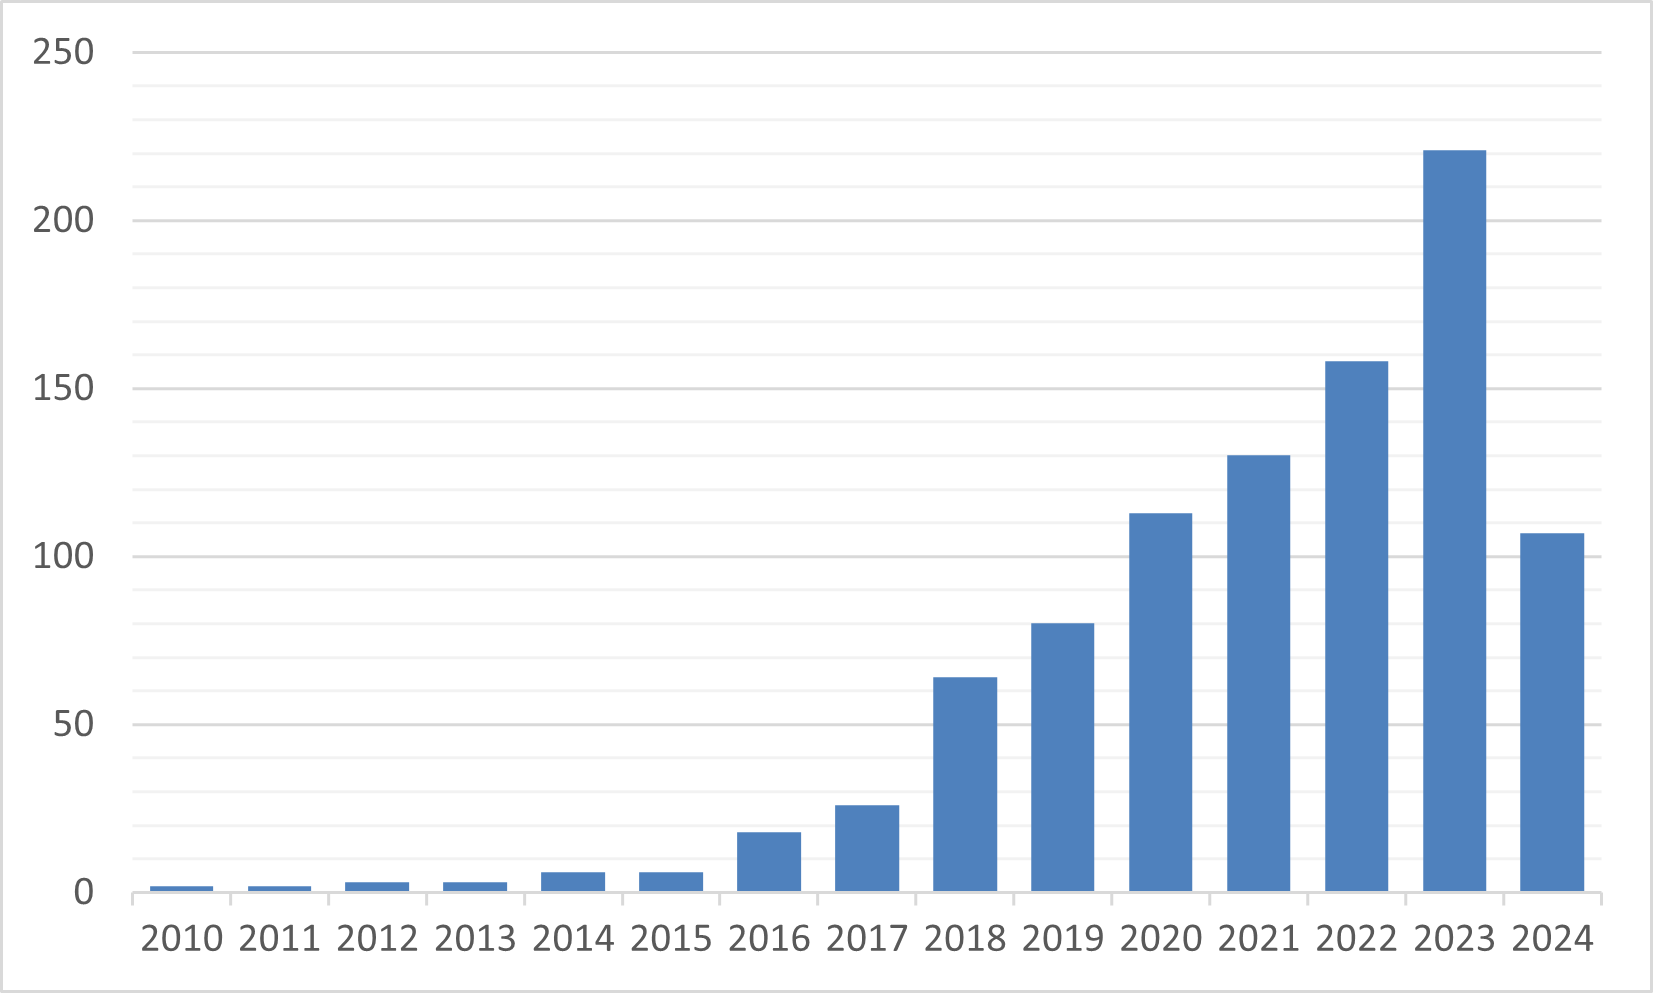
\includegraphics[scale=0.6]{../Resources/Growth in ML enabled devices.png}}
    \caption{Number of FDA-approved AI/ML-enabled medical devices since 2010} 
    \label{fig:FDA}
\end{figure}

\subsubsection{Radiology}
In radiology, machine learning is a powerful tool that can help physisicians with CT scan and MRI scan to diagnose diseases and extract latent insights from the scans. Some example work include
\begin{itemize}
    \item Classification of triple negative breast canser using ultrasound images \cite{wu_machine_2019}
    \item Detection of pulmonary lung nodules from CT scans by convolutional neural network \cite{van_ginneken_off--shelf_2015}
    \item Pneumonia detection from chest X-rays using modern deep learning \cite{rajpurkar_chexnet_2017}
    \item Detection of breast mass from mammography scans using convolutional neural networks \cite{arevalo_convolutional_2015}
\end{itemize} 



\subsubsection{Dermatology}
In dermatology diagnosis, visual inspection remains the prominent method for determining the severity of a skin abnormalities or lesions. 
Machine learning emerges as an effective automation method as they learn the latent features that differentiate between benign and malignant lesions in skin melanoma. 
As early as 1994, the research in \cite{ercal_neural_1994} applied neural network to automate the classification of malignant melanoma from melanoma-like benign tumors.
The model was given the discriminant characteristics such as tumor shape and relative color, manually extracted from digital images of skin cancer.
In \cite{esteva_dermatologist-level_2017}, a convolutional neural network was trained on 100,000 clinical images of skin cancer and achieved an accuracy similar to that of a dermatologist.
Once these models have been trained extensively on computationally efficient hardware, they can be packaged and deployed on mobile devices to make inferences on skin lesions. 
This can further increase the accessibility of machine learning functionalities to the wider population.



\subsubsection{Hematology}
In the case of hematological diseases, early prediction can help prevent progression and complication of blood disorders such as leukemia and lymphoma. 
Traditionally, practitioners diagnose hematological conditions by cytomorphologic phenotypic assessment of peripheral blood (PB) and bone marrow (BM) samples.
Newer techniques for disease diagnosis includes flow cytometry and molecular genetic analyses. 
However, diagnostic ambiguity often occurs in such manual process depending on the operator experience and capabilities. 
The reproducibility of clinical results suffer from inter- and intravariations amongst skilled hematologists and pathologists \cite{walter_artificial_2023,wu_hematologist-level_2020}.
Therefore, there needs to be an automated process for reduced reliance on expert knowledge and increased consistency in data interpretation.
Given its predictive power, machine learning implementation in disease diagnosis from blood samples is an active research topic.

In 2014, early developments of automated ML systems for cytomorphologic assessment had limited capabilities, performing tasks such as blood cell counting or classificiation of lymphoid cell types \cite{alomari_automatic_2014,alferez_automatic_2014,alferez_automatic_2015}.
In \cite{guncar_application_2018}, two ML models were developed to predict hematologic disease.
One of them was trained on all available blood test parameters and the other trained on a reduced set of parameters usually obtained from patient admittance.
When this input is paired with the knowledge of the five most likely diseases, the models achieve predictive performance on par with haematology specialists.
In a research by \textit{Wu et al.} \cite{wu_hematologist-level_2020}, the researchers developed a BMSNet with the YOLO-v3 CNN architecture to assist in BM smear interpretation.
The model performance was reported as comparable to that of expert hematologists and pathologists in various tests, except for the classification of myelodysplastic cases.
\textit{Matek et al.} \cite{matek_highly_2021} automated cytomorphologic examination of BM smears by training two CNN-based classifiers. 
The first model has the ResNeXt-50 architecture, previously used in \cite{matek_human-level_2019} for recognition of acute myeloid leukemia blast cells from PB smears due to its low number of hyperparameters.
The second model was a sequential CNN models with a simpler architecture for baseline performance comparison.
The research in \cite{cheuque_efficient_2022} employed a two-stage CNN architecture to classifies four types of white blood cells (leukocytes).
The first layer of CNN leveraged a Faster R-CNN network to delineate the regions of interest and differentiate mononuclear cells from polymorphonuclear cells. 
The seconds layer consists of two parallels CNN with the MobileNet architectures and transfer learning to further categorize the subclasses of leukocytes. 
The lightweight architecture and parallelization in the second layer allows for faster inferencing time.

Flow cytometry or multiparameter flow cytometry (MFC) is a modern techniques for routine blood analysis and an enabling factor for AI integration in hematology.
Modern MPC can analyze thousands of cells a second to generate a large dataset of high dimensional data \cite{walter_artificial_2023}. 
Although this appears challenging for human interpretation and emphasizes the reliance on expert knowledge, a machine learning algorithm can be trained to interpret the latent representation and correlation in the flow cytometry data.
The researchers in \cite{zhao_hematologist-level_2020}, leveraged machine learning by first converting MPC data into multicolor 2D images using a self-organizing map before feeding this data representation through a CNN architecture for classification.
The developed model was capable of categorizing healthy cells from diseased ones, as well as the seven subclasses of mature B-cell neoplasm.

\subsubsection{Ophthamology}
In the field of ophthamology, a fundoscopy is a non invasive procedure for inestigating the patient's fundus, or the back of their eyes, to diagnose vision conditions and risk factors leading to vision loss.
These detected factors can be used to predict the onset of diseases such as diabetic retinography, glaucoma, retina neoplasms, and macular degeneration \cite{kumar_artificial_2023}

\textbf{Diabetic retinography (DR)} is a condition where high blood sugar level causes damaged vessel in the retina. 
This condition is one of the common causes of vision loss and impairment amongst American living with diabetes and working age adults \cite{commissioner_fda_2020,abramoff_pivotal_2018}.
In 2018, the FDA approved of IDx-DR, the first AI-enabled system for detecting DR.
The research in \cite{abramoff_improved_2016} and \cite{abramoff_pivotal_2018} leveraged a multilayer CNN to train independent detectors for the anatomy and the characteristics of DR, including microaneurysms, hemorhages, and lipoprotein exudates.
The results of these detectors are combined to return the levels of the diseases. 
The study in \cite{sayres_using_2019} implemented an Inception-v4 CNN architecture, to detect the severity grade of DR and provide a heatmap of regions of interest.

Researchers have also integrated AI into the early diagnosis of \textbf{age-related macular degeneration (AMD)}, a chronic and irreversible condition and one of the most common cause of central vision loss. 
One characteristics that signals the onset of AMD is the appearance of hard or soft drusen on optical coherence tomography (OCT) images or color fundoscopy images.
ML can automate the drusen detection to diagnosie early signs of AMD, such as in \textit{Burlina et. al} \cite{burlina_automated_2017} where they employed Deep CNN on color fundus images. The network employs transfer learning on the AlexNet structure, which includes dropout lauers, ReLU activation, and normalization. The weights was trained using stochastic gradient descent and Nesterov momentum, and a learning rate of 0.001 for 50 epochs. This model was compared to a pretrained Overfeat DCNN (New York University) with a linear SVM for classification. The results showed comparable performance to expert human graders, with accuracy ranging from 88.4\% and 91.6\% and an ROC-AUC score betwen 0.94 and 0.96.
In the research done by \textit{Schlegel et al.} \cite{schlegl_fully_2018}, the authors adopted an autoencoder architecture and CNN for learning a simplified representation of the raw images (\autoref{fig:Schlegl_OCT_autoencoder} shows the architecture of this network). The encoder portion of this networks generates an optimized abstract representation of the data embedding, which is then used to re-generate a corresponding image with class labels.

\begin{figure*}[h]
    \centering{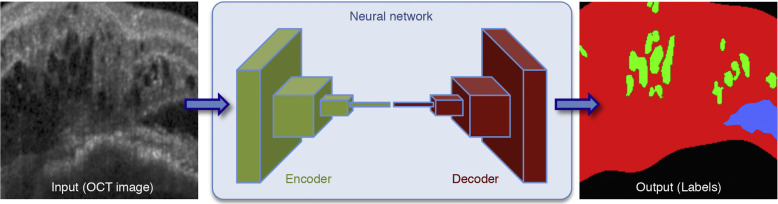
\includegraphics[scale=1.0]{../Resources/Schlegl_OCT_autoencoder.jpg}}
    \caption{The proposed network with an autoencoder architecture using CNN in the encoder portion to form a simplified representation of the input features} 
    \label{fig:Schlegl_OCT_autoencoder}
\end{figure*}

\textbf{Glaucoma} is another medical condition resulting in damaged optic nerve. The condition happends when there is a blockage preventing the drainage of the aqueous humor fluid and leading to pressure build-up in the eye.
In \textit{Shibata et al.} \cite{shibata_development_2018}, the authors developed a deep residual network (ResNet) for glaucoma detection from 2D fundus photography. The network is based on the CNN architecture with residual connections to prevent the gradient vanishing and gradient divergence problem, thus allowing for more effective training of deeper networks.
In a recent study by \textit{Thompson et al.} \cite{thompson_assessment_2020}, the authors implemented a deep learning solution for glaucoma detection using B-scan from OCT images. This reseach employed a residual deep convolutional neural network (ResNet34) and transfer learning to leverage the previously trainined feature extraction layers on the ImageNet dataset.


\subsubsection{Oncology}
The integration of AI and ML systems in cancer treatment is an active branch of research.
Some potential use cases of AI in this field of research are radiotherapy dosage optimization and image segmentation for tissue abnormality detection. AI algorithms have shown promising improvements compared to manual planning in these fields \cite{thompson_artificial_2018}.
In radiation treament, the prescribed dose is determined by specialist prior to initial treatment. This knowledge base planning approach depends on dose histograms and historical patient plans. However, the variations in tumour biology poses challenges to this process as the dosage can significantly vary. Further complication may arise depending on the location of the tumour and surrounding organs, thus preventing the desired doseage delivery \cite{huynh_artificial_2020}. In this sense, AI methods can personalize the treatment plan and the optimal prescription achievable depending on the contour of the tumour and organs.

In \textit{Nguyen et al.} \cite{nguyen_feasibility_2019}, the authors leveraged the modified U-net CNN network (\autoref{fig:U-Net_architecture_cancer_dose}) to achieve contour-to-dose mapping. The U-Net architecture was first introduced in \cite{ronneberger_u-net_2015} for image segmentation task. In a U-Net, the compressed representation of image data that was learned in the \textit{contracting path} undergoes up sampling and up-convolutions in the \textit{expansive path}. The features in the expansive path are combined with high-resolution feature from the contracting path to create the segmented representation.

\begin{figure*}[h]
    \centering{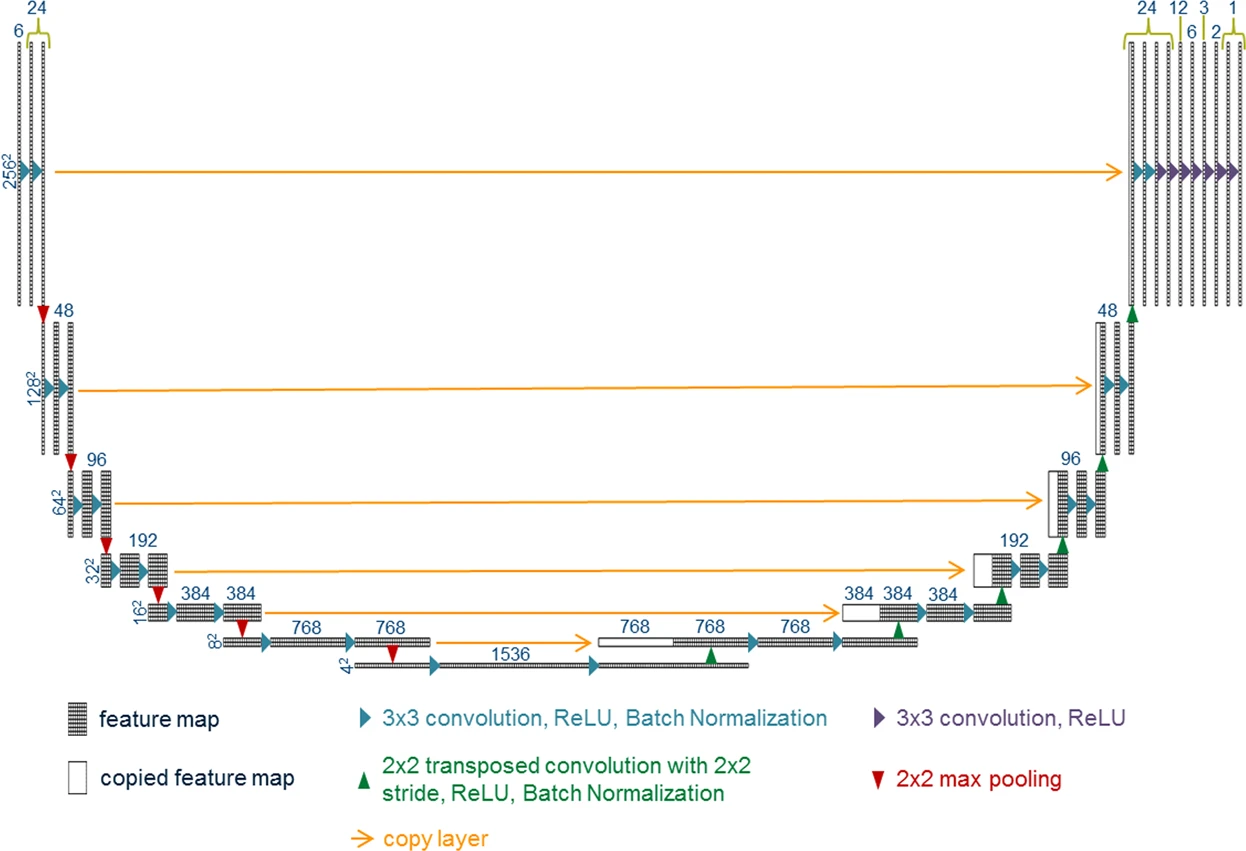
\includegraphics[scale=0.3]{../Resources/U-Net CNN Architecture.png}}
    \caption{Modified U-Net architecture for personalized prostate cancer dosage prescription based on patient anatomy}
    \label{fig:U-Net_architecture_cancer_dose}
\end{figure*}



\section{Challenges}
\subsection{Trust}
\subsection{Accountability}
\subsection{Data privacy and protection}
AI technologies depend on a vast amount of patient data and record to make accurate predictions when subjected to unseen data.
However, in the event of a database violation or data breach, confidential patient information can be exploited for malicious intentions (identity theft, social stigma, discrimination,...).
This can put a mental burden on the patient suceptible to the violation and other relevant stakeholders.
Therefore, adequate law and guidelines are crucial to regulate the application of AI in medical and prevent misuse of data


The data gathering and handling of health data in the US is controversial, raising legal and ethical privacy questions \cite{price_privacy_2019}.
Although the data can originate from various sources, such as healthcare providers, insurance claim, and wearable devices, US privacy law operates in different extents depending on the data source.
This law also depends on the custodian of the data. Under the Health Insurance Portability and Accountability Act (HIPAA), the federal Privacy Rule only governs data handling between the conventional entities, such as healthcare providers, health insurance provides, patients, and intermediaries. 
However, \cite{price_privacy_2019} pointed out existing gap in HIPAA regulation.
Although, HIPAA protect patient privacy from health data breach via a deindentifying process, patient data can be reidentified through data triangulation from other datasets.


Furthermore, a more fundamental problem is the amount of health related data not regulated under HIPAA \cite{price_privacy_2019}. 
Originally enacted to regulate data privacy in health records and between covered entities, HIPAA does not account for health data generate outside the confinement of these covered entities. 
In the big data world, tech companies are displacing covered entities in the collection of health information and personal data from online searches, application logs, and smart wearable devices.

\section{Case Study: From Turing Award to Nobel Prizes}
Artificial intelligence (AI) and machine learning (ML), two transformative forces within computer science, are undeniably making rippling effects into other traditional technological fields. The prestigious 2018 Turing Award honored Geoffery Hinton, a trailblazer in artificial neural network, for his earlier pioneering work that paved the way for recent AI developments. This landmark achievement highlighted the fundamental role of AI in advancing computer science and unravelling the complexities of natural systems-a contribution that recently earned Hinton the 2024 Nobel Prize in Physics. Shortly after Hinton's recognition, Demis Hassabis and John Jumper, two Google DeepMind executives, received the Nobel Prize in Chemistry for their pioneering contributions to decoding microscopic protein structures in the AlphaFold project.
Using advanced AI-driven approaches, they created solutions capable of predicting protein folding—a pivotal biological challenge as a protein’s structure directly determines its function within cells and organisms. This AI breakthrough has fundamentally transformed biochemistry, enabling rapid drug discovery, personalized medicine, and a deeper understanding of cellular mechanisms.

\subsection{History of AlphaFold Development}

The first version of AlphaFold \cite{senior_improved_2020} made its debut at the 13th Critical Assessment of protein Structure Prediction (CASP13), a global competition that evaluates the latest methods for predicting protein structure. This task is known for its complexity due to the vast number of potential ways protein chains can fold. AlphaFold introduced an innovative approach that combined deep neural networks with reinforcement learning to predict the 3D structure of proteins with higher accuracy than previous methods. The algorithm uses a multiple sequenece alignment technique (MSA) to process protein sequence data and related evolutionary data to understand amino acid relationship. This techniques provides information about conserved amino acids accross similar proteins and offers clues of possible protein folding structure. AlphaFold’s CNN architecture analyzed these features, learning patterns in amino acid interactions and generating predictions on the likely contacts between amino acid pairs. After initial training, AlphaFold employed reinforcement learning techniques to refine predictions iteratively, adjusting the protein’s structure until it reached a stable conformation. By rewarding predictions that brought the structure closer to plausible physical conformations, AlphaFold improved the reliability of its results over successive iterations.

AlphaFold 2 was a major leap forward and was presented at CASP14 in 2020. This version used a new architecture that relied heavily on attention mechanisms, allowing it to focus on relationships between amino acids and to understand how they influence a protein’s folding process \cite{jumper_highly_2021}. The approach resembled “transformer” models commonly used in natural language processing, which helped AlphaFold 2 capture intricate dependencies within protein \autoref{fig:AlphaFold2}. The two main attention pathways - pairwise interation representation and evoformer block - were introduced to help the model analyzed these long-range dependencies. The first attention architecture provides understanding on amino acids interaction within the folded structure, while the second pathway is a series of transformer layers that compbine both sequence information and the pairwise interaction data to build a cohesive representation of the protein's 3D structure. The algorithm further refines its prediction iteratively given the physical constraints and previous predictions and produce progressively more accurate predictions. The AlphaFold 2 algorithm achieve to an average accuracy comparable to experimental methods for many proteins.

\begin{figure*}[h]
    \centering{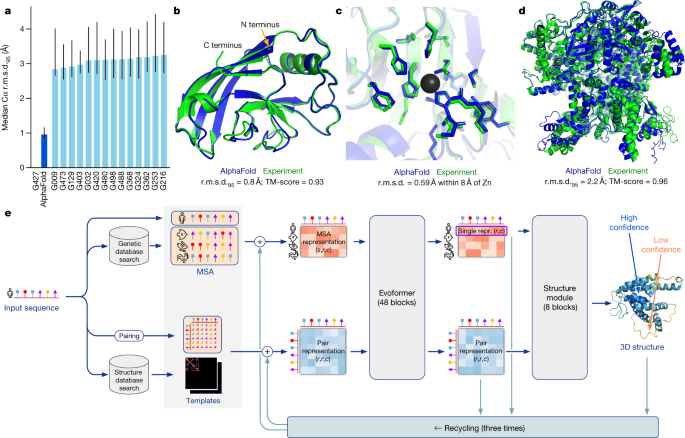
\includegraphics[scale=0.6]{../Resources/AlphaFold 2.png}}
    \caption{Architecture of AlphaFold 2} 
    \label{fig:AlphaFold2}
\end{figure*}


As many biological functions are carried out by protein complexes, DeepMind introduced AlphaFold-Multimer v2.3, an extension designed to predict the structure of protein complexes (multimers) rather than individual proteins. This version builds on AlphaFold 2’s framework, adapting it to better handle interactions between multiple protein chains, which are crucial in many biological processes.

Compared to AlphaFold 2 and AlphaFold Multimer, which can model protein monomers and protein complexes, AlphaFold 3 was capable of modeling the interaction amongst a wider range of biomolecules such as ligands, nucleic acids, and modified residues \cite{abramson_accurate_2024}. AlphaFold 3 introduced a  2 new modules: 1) the pairformer module to reduce the complexity of MSA processsing, and 2) the diffusion module to directly predict atom coordinates by gradually improving local structures without the sterochemical constraints required in the AlphaFold 2 approach (). In AlphaFold 3. 
The pairformer block replaces the evoformer and the algorithm only operates on the pair representation and the single representation.

\begin{figure*}[h]
    \centering{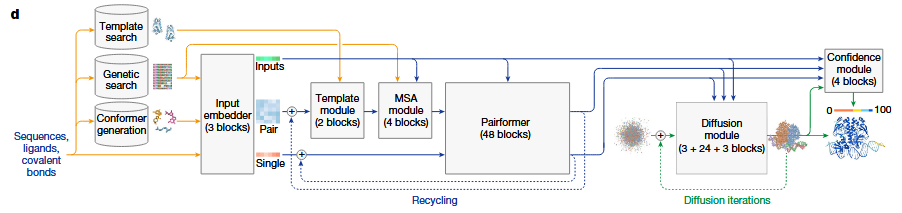
\includegraphics[scale=0.7]{../Resources/AlphaFold_3.png}}
    \caption{AlphaFold 3 architectures} 
    \label{fig:AlphaFold3_Architecture}
\end{figure*}

\subsection{Implications}
As can be seen from this case study, the implementaion of AI and ML in healthcare is a promising research direction. The implications of AlphaFold 3 and similar rapid advances in AI for modern medicine are profound, as they signal a new era of data-driven, precise, and personalized healthcare solutions. As AlphaFold 3 is capable of predicting thei nteraction between proteins and other molecules, researchers can quickly find binding sites for potential drugs and provide a methodical framework for drug design. In other scenarios, researchers can design more effective vaccine with knowledge of antibody-antigen interactions. This is invaluable in speeding up intial stages of vaccine development with reduced time between pathogen identification and vaccine candidate selection  






% Bibliography/Reference Stuff
\bibliography{minh}
\end{document}